\setcounter{section}{3}

\section{基于攻防行为可区分性的恶意软件家族分析}
\label{sec:family-analysis}

第三章构建的三层知识库与大语言模型语义识别流水线，为家族层面的行为比较提供了统一的表征基础。在此基础上，本章不再停留于单个样本的检测性能，而是进一步考察不同勒索软件家族在攻防行为组合、函数调用图组织方式以及知识证据覆盖模式上是否存在稳定且可重复的差异结构。与面向分类器性能的实验不同，本章的目标是以统计分析揭示家族可区分性的客观形态，为后续识别模型的结构设计提供经验支撑，而非事后给出单一路径的因果性解释。

本章围绕样本级行为画像、调用图关键路径以及三层知识特征三个层面展开分析。具体而言，首先从 34 个家族、437 个勒索软件样本中归纳七类攻防行为的分布差异，考察家族在攻击性与防御性极性空间中的占位方式；随后对函数调用图及其攻击性、 防御性子图进行拓扑比较，分析家族间结构模式是否具有统计稳定性；最后审计词法层、语义层与统计层在不同家族上的覆盖强度和判别能力，以验证第三章分层知识设计的必要性。

\subsection{问题分析}

\subsubsection{恶意软件家族行为分析的研究背景}

恶意软件研究长期以“是否为恶意样本”为核心判别目标，典型工作从权限与 API 特征建模出发，逐步发展到原始字节序列学习与端到端深度识别 \cite{arp2014drebin,raff2017learning}。对于勒索软件而言，这类研究有助于提升检测精度，但难以直接回答另一个同样关键的问题：具有共同来源、共同工具链或共同运营模式的家族，是否在行为组织上呈现稳定结构。家族层面的规律一旦能够被稳定观测，就不仅可以解释不同家族的行为风格差异，还能够为后续检测模型提供更具结构性的先验。

已有少量研究从家族视角切入勒索软件分析。例如，Cicala 等围绕密钥生成机制比较了不同勒索软件家族的加密实现差异 \cite{cicala2020analysis}，Hou 等对勒索攻击中的数据破坏模式进行了实证梳理 \cite{hou2024empirical}，Tang 等则从检测流程角度讨论了勒索软件的多阶段证据整合问题 \cite{tang2020ransomspector}。这些工作说明，家族差异不仅存在于表层的样本标签之中，也体现在加密方式、执行路径和系统破坏策略等更深层的行为组织上。然而，现有成果大多聚焦单一机制或单类证据，尚未形成一个同时覆盖语义行为、调用图结构和多层知识命中的统一分析框架。

\subsubsection{现有家族分析方法的局限性}

现有家族分析方法至少存在四方面不足。第一，多数工作仍采用代码相似度、字符串重合率或扁平化统计特征作为主要比较依据。这类证据虽然便于批量处理，但更适合回答“样本是否相似”，不擅长刻画“相似样本为何在行为组织上相似”。对于使用不同编译链、不同混淆策略乃至不同语言实现的现代勒索软件而言，仅依赖代码表层特征很容易低估跨家族差异，也难以解释家族内部的一致性来源。

第二，现有分析往往将恶意行为视为单一整体，而未显式区分攻击性行为与防御性行为。事实上，加密、文件遍历、勒索信展示等攻击性动作面向载荷执行，而混淆、环境检测、延迟执行、系统破坏等防御性动作则服务于逃逸与持久化。两类行为在功能目的、触发条件和组织方式上并不相同。如果将其压缩为单一路径或单一统计量，模型能够获得的只是“恶意性强弱”的粗粒度判断，而不是“家族如何组织攻击与规避”的结构化知识。

第三，家族分析往往忽略了调用图中的关键路径差异。勒索软件并不是一组相互独立的函数标签，而是一套在执行时序中逐步展开的行为系统。攻击性逻辑可能分布在多条并发或分支路径上，而防御性逻辑常常集中在少数关键节点附近。若不引入调用图拓扑信息，仅以样本级统计值比较家族，很难解释家族差异到底源于行为内容本身，还是源于行为在程序结构中的组织方式。

第四，分层知识体系的家族覆盖能力尚缺乏实证审计。第三章提出的词法层、语义层与统计层分别从字面证据、语义证据和数值证据三方面描述恶意软件，但这些证据在不同家族上是否具有一致覆盖、是否存在互补关系、哪一层对哪些家族更重要，仍需要通过系统比较加以证明。若缺乏这一层面的分析，知识库设计虽然在工程上可用，却难以形成充分的学术说服力。

\subsubsection{本章研究目标与技术路线}

基于上述不足，本章将家族分析组织为三个递进层面。首先，在语义行为层面考察不同家族在七类攻防行为上的分布差异，验证行为画像是否足以形成紧凑而可解释的家族表征；其次，在程序结构层面比较函数调用图及攻击性、 防御性子图的拓扑差异，观察家族间是否存在稳定的关键路径模式；最后，在知识证据层面对三层知识库的覆盖强度和判别力进行审计，明确各层在家族分析中的独立贡献与互补价值。

需要说明的是，本章的结论定位为“统计支撑”和“经验支撑”。也就是说，本章并不声称第五章的模型结构只能由本章结论唯一推导出来，而是通过家族级证据说明：将攻击性与防御性信息分离建模、将调用图结构与数值特征联合建模，具有明确的数据基础和合理的工程动机。

\subsection{PolarProfile：知识驱动的多粒度行为画像框架}

\subsubsection{知识驱动的多粒度行为画像设计思路}

为在家族层面统一比较不同样本，本章构建 PolarProfile 框架，将第三章得到的函数级行为标签、样本级统计特征与调用图结构进一步组织为可分析的多粒度画像。其核心思想是，将原本分散在函数、样本和家族三个尺度上的证据显式对齐：先在函数粒度识别行为，再在样本粒度聚合为画像向量，最后在家族粒度形成可比较的分布统计。

设样本 $s$ 的七类行为占比向量为 $\mathbf{b}(s)$，其中前三维对应攻击性行为，后四维对应防御性行为，则样本的行为画像可形式化为

\begin{equation}
\mathbf{b}(s)=\left[p_{1}(s),p_{2}(s),p_{3}(s),p_{4}(s),p_{5}(s),p_{6}(s),p_{7}(s)\right],
\end{equation}

其中，$p_i(s)$ 表示样本 $s$ 中第 $i$ 类行为函数占全部已标注函数的比例。进一步地，定义攻击性强度 $O(s)$ 与防御性强度 $D(s)$ 为

\begin{equation}
O(s)=\sum_{i=1}^{3}p_i(s), \qquad D(s)=\sum_{i=4}^{7}p_i(s).
\end{equation}

由于单个函数可能同时命中多类行为标签，因此 $\sum_{i=1}^{7}p_i(s)$ 不必等于 1，$O(s)$ 与 $D(s)$ 也允许同时处于较高水平。换言之，极性空间并不用于刻画互斥分布，而是用于刻画攻击性与防御性证据在同一样本中的并存强度。

在家族粒度上，设家族 $f$ 的样本集合为 $S_f$，则该家族的平均行为画像定义为

\begin{equation}
\bar{\mathbf{b}}_f=\frac{1}{|S_f|}\sum_{s\in S_f}\mathbf{b}(s).
\end{equation}

其中，$|S_f|$ 为家族 $f$ 的样本数，$\bar{\mathbf{b}}_f$ 表示该家族在七类行为上的平均结构。通过上述定义，函数级、样本级和家族级证据被统一映射到同一分析空间，为后续统计比较提供基础。

\subsubsection{三阶段工作流}

PolarProfile 的实现过程分为三个阶段。第一阶段为二进制智能提取。对 437 个带家族标签的 PE 样本进行脱壳、反编译和调用图导出，得到函数级伪代码、全局常量以及 GDL 格式的函数调用关系图。第二阶段为多层行为证据识别，利用第三章构建的三层知识库分别提取词法命中、语义命中和统计特征，并结合上下文感知行为精炼，对函数进行七类行为标注。第三阶段为多粒度行为画像构建，将函数级标签进一步聚合成样本级行为画像、攻击性/防御性极性坐标和子图拓扑统计，再在家族级进行分组汇总。

该三阶段流程的关键价值在于，它将知识驱动的行为识别与结构驱动的图分析统一到了同一数据链路中。前两阶段负责把程序语义转化为可计算的行为证据，第三阶段则将这些证据从“单个函数的局部现象”提升为“家族级分布规律”。因此，本章关注的不是某个函数是否加密，而是整个家族在加密、遍历、规避和破坏等行为上的组合方式及其稳定性。

\subsubsection{输出数据集}

围绕上述流程，本章最终形成三类核心分析对象。其一是样本级行为画像矩阵，用于描述七类行为占比与攻击性/防御性极性分布；其二是样本级调用图与攻击性、 防御性子图拓扑统计，用于分析家族的关键路径组织模式；其三是三层知识库命中记录与 54 个可比较统计特征，用于审计不同家族在词法、语义与数值层面的覆盖强度和判别能力。与仅保留单一分类标签的传统数据集不同，这些输出保留了家族分析所需的解释性信息，因此能够支撑更细致的统计论证。

\subsection{家族谱系总览}

\subsubsection{实验数据集构成}

本章分析对象为 34 个勒索软件家族的 437 个样本，不设置样本量过滤门槛，而是对全部家族进行完整纳入。样本分布呈现明显的长尾特征：BlackCat、Kovter、WannaCry、TeslaCrypt、Hive 和 Bianlian 分别包含 47、45、43、35、33 和 26 个样本，构成数据集中的主要家族簇；与此同时，Akira、Matsnu、Maze、Rhysida、Royal 等家族样本量较少，承担对小样本家族可区分性的补充观察。对这类长尾分布，本文不采用简单剔除策略，而是在解释具体家族现象时明确说明样本规模对结论稳健性的影响。

\subsubsection{家族谱系分布概览}

如图~\ref{fig:family-phylogeny} 所示，34 个家族在时间分布、技术路线与行为侧重点上表现出明显异质性。早期家族更多体现为围绕 Windows 系统 API 的直接加密和文件遍历逻辑，而 2020 年之后的现代 RaaS 家族则更倾向于采用模块化组织方式，在加密载荷之外同时引入环境检查、延迟执行和系统破坏等规避动作。这一趋势意味着家族差异并不仅仅来自“是否加密”，而来自“如何组织攻击与规避”这一更高层级的行为策略。

\begin{figure}[htbp]
\centering
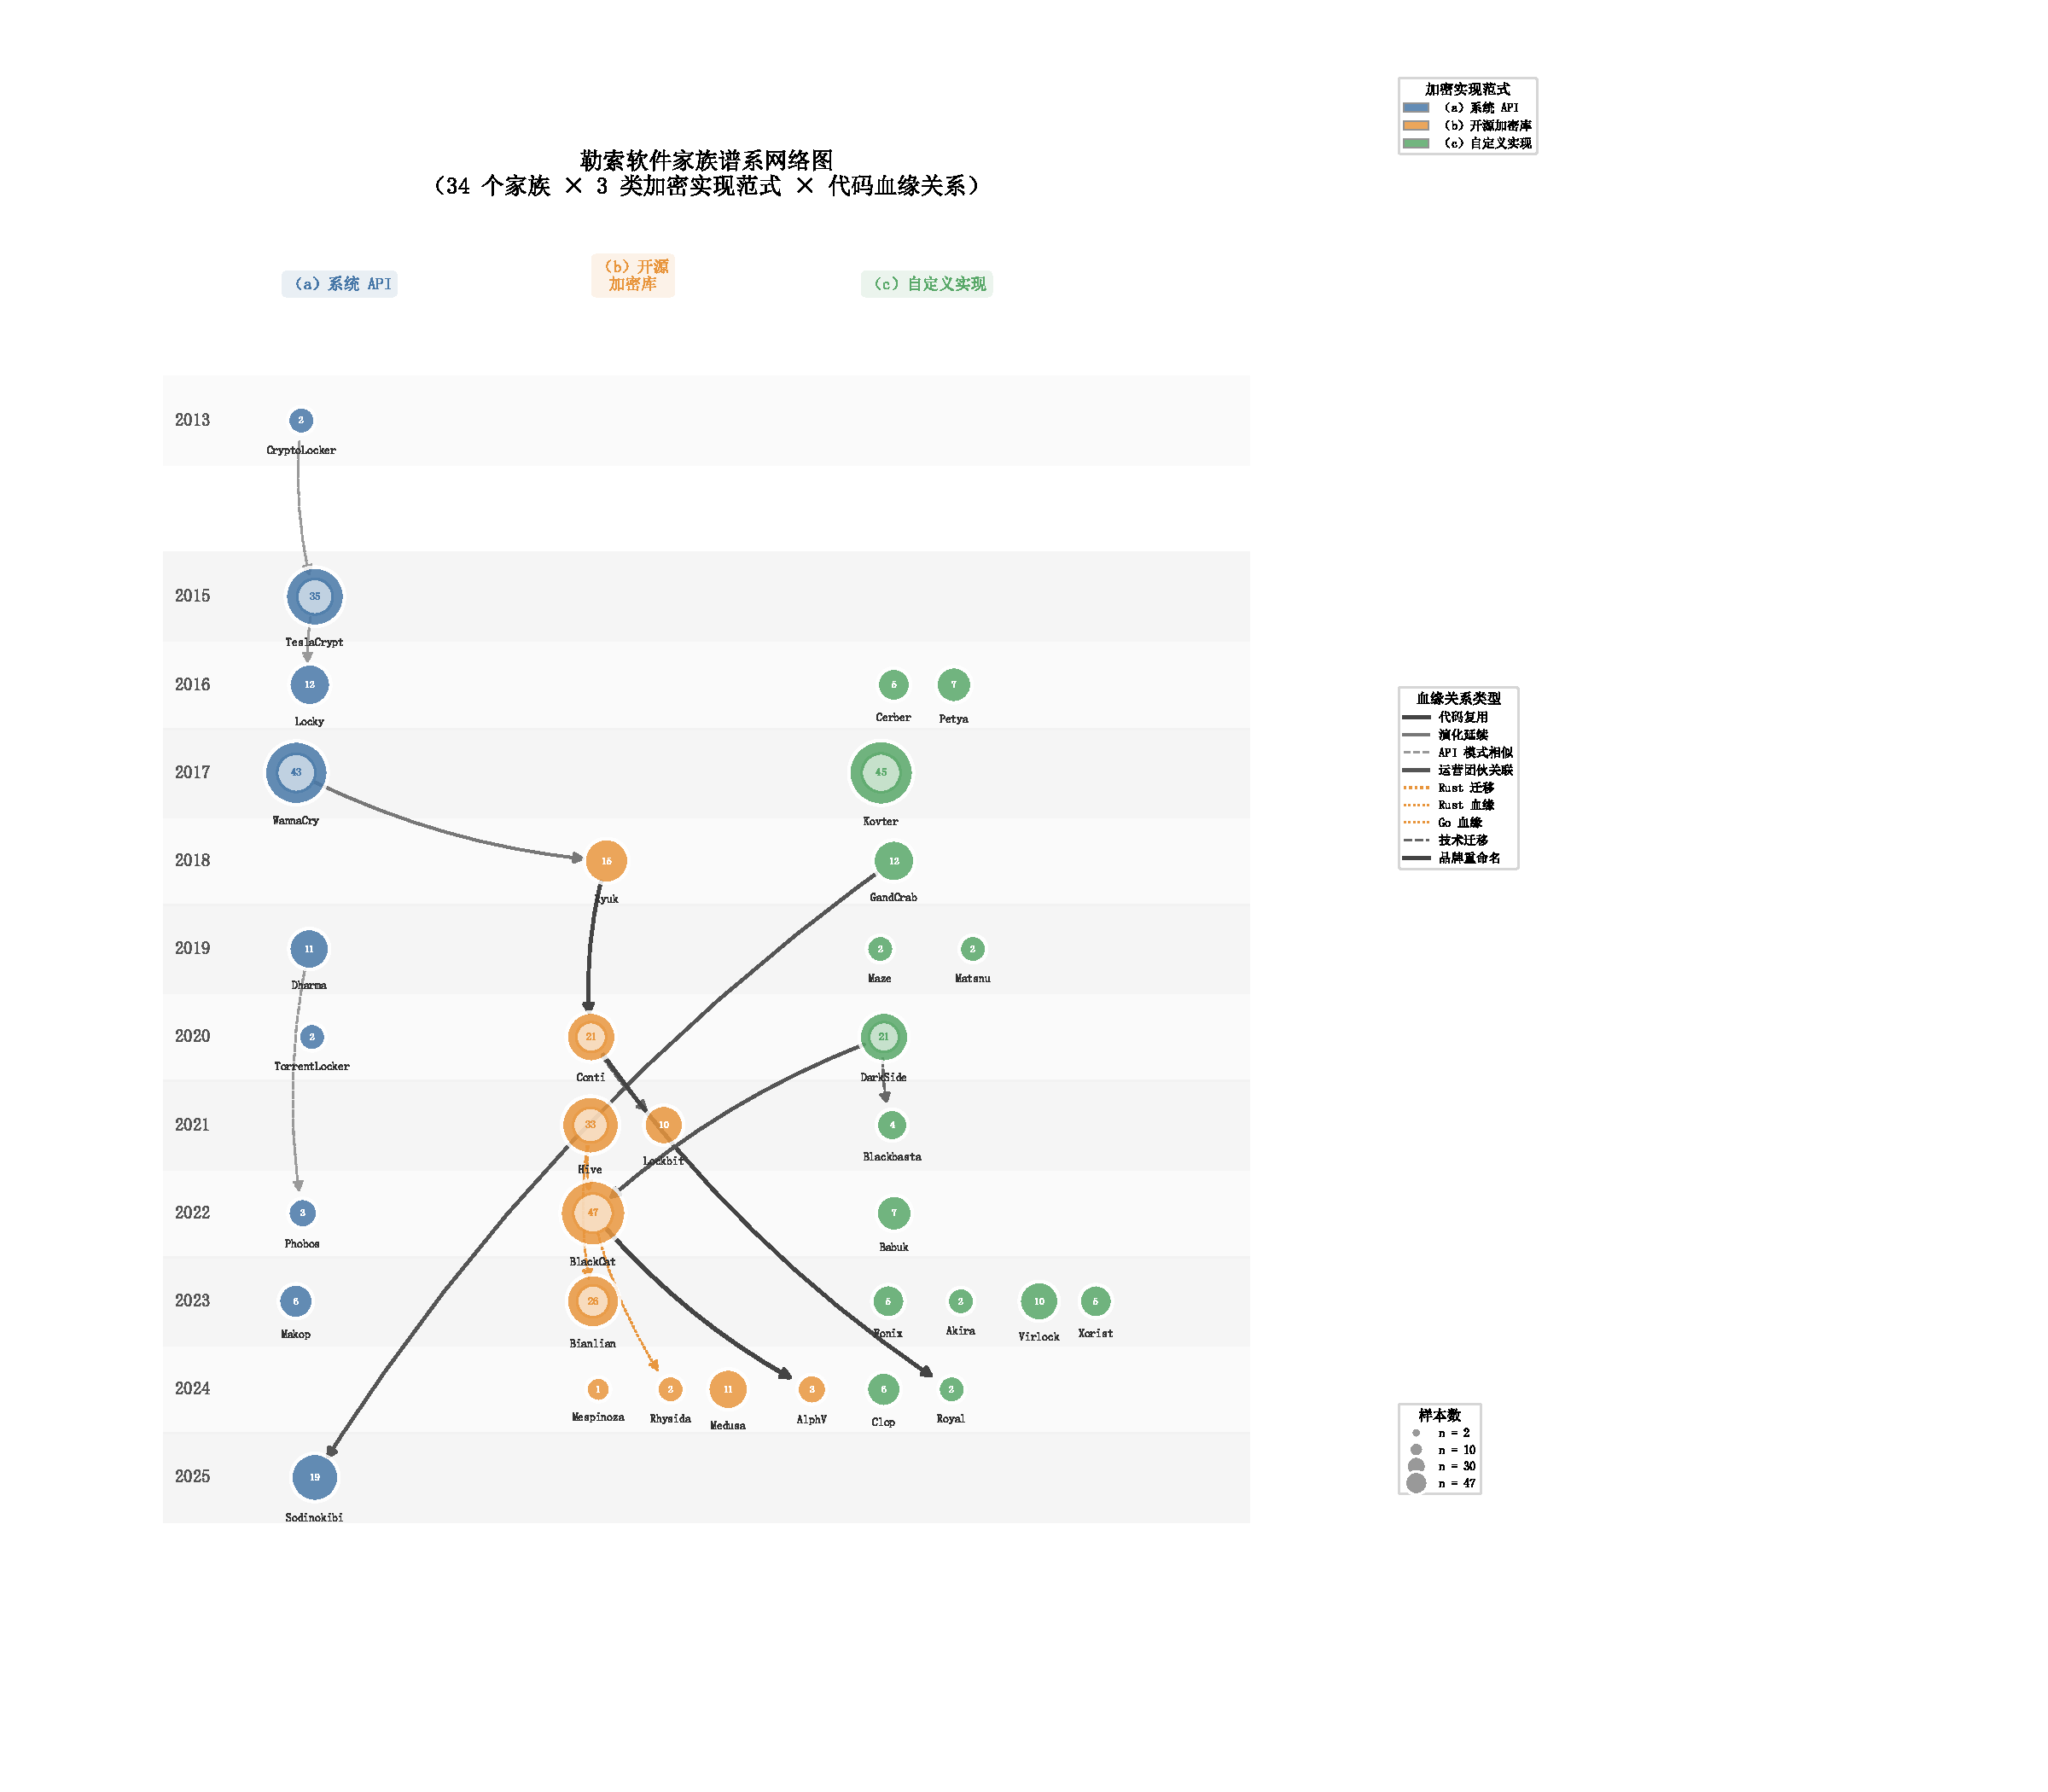
\includegraphics[width=0.95\linewidth]{figures/fig_04_family_phylogeny.pdf}
\caption{勒索软件家族谱系网络图}
\label{fig:family-phylogeny}
\end{figure}

图~\ref{fig:family-phylogeny} 反映出两个值得强调的事实。首先，家族演化并不是简单的时间线叠加，而是不同技术路线长期并行：一类家族保留明显的系统 API 驱动特征，另一类家族则向库化、模块化和多语言实现迁移。其次，家族谱系网络中的“邻近性”并不总意味着相同的攻击强度，而更常表现为实现范式或规避策略的相似，这也是本章必须同时引入行为画像、图结构和统计特征三个层面的原因。

\subsubsection{加密实现范式分类}

结合反编译结果和第三章的知识库命中记录，34 个家族的加密实现大体可以归纳为三种范式。第一类为操作系统 API 主导型，以 WannaCry、TeslaCrypt、Dharma 等家族为代表，其加密路径通常围绕典型的 CryptoAPI 调用链展开。第二类为开源加密库复用或定制型，以 Conti、Ryuk、Lockbit、BlackCat、Hive 和 Bianlian 等家族为代表，这类样本往往在伪代码中保留更明显的 OpenSSL、Rust crate 或 Go 标准库调用痕迹。第三类为自实现加密函数主导型，以 DarkSide、GandCrab、Babuk、Xorist 和 Petya 等家族为代表，其加密逻辑更多以位运算、查表和轮函数形式嵌入程序主体。

这一划分与第三章三层知识库的设计形成了直接对应关系：词法层对第一类家族更敏感，语义层更擅长识别第二类家族中的库级语义模式，而统计层则对第三类家族中的位运算密度、节区熵和控制流复杂度更为敏感。因此，家族的加密范式差异并不是独立于知识库设计之外的背景信息，而是三层证据互补性的现实来源。

\subsubsection{代码血缘关系与攻防极性概览}

除加密范式之外，不同家族在代码血缘和行为极性上也表现出值得关注的结构特征。部分家族沿用了相近的工具链和模块化框架，因而在全图规模、度分布和聚类系数上表现出相似的结构外观；另一些家族虽然在代码相似度上并不突出，但在攻防极性空间中占据接近区域，说明其运营策略具有相似性。需要强调的是，本章不试图重建严格的家系树，也不将视觉聚类结果视为核心证据，而是将这些谱系信息作为理解后续统计差异的背景参照。

\subsection{家族攻防行为画像差异分析}

为了比较家族在语义行为层面的差异，本节以样本级七维行为画像为基础，对 34 个家族进行非参数统计检验。考虑到各家族样本规模不均、行为占比不服从正态分布，本文采用 Kruskal--Wallis 检验衡量家族间差异，并使用效应量 $\eta^2$ 评价差异的实际大小。与此同时，结合攻击性强度与防御性强度构造二维极性空间，以考察家族在行为组合方式上的整体分布。

\begin{figure}[htbp]
\centering
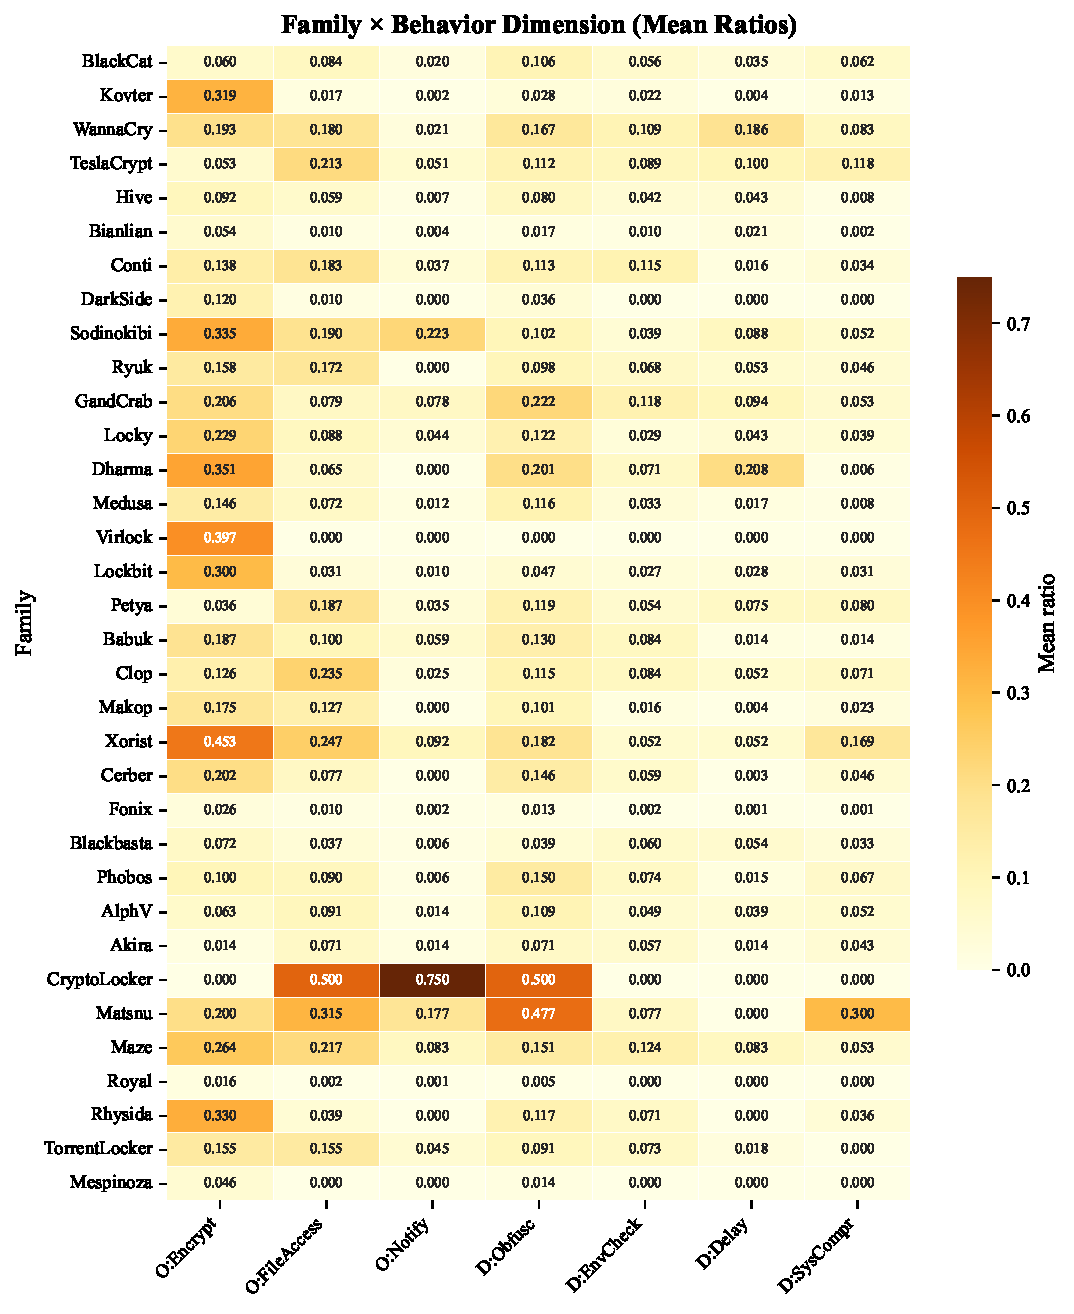
\includegraphics[width=0.95\linewidth]{figures/fig_04_rq1_behavior_heatmap.pdf}
\caption{家族攻防行为画像热力图}
\label{fig:family-behavior-heatmap}
\end{figure}

如图~\ref{fig:family-behavior-heatmap} 所示，不同家族在七类行为维度上的热度分布并不均匀，而是形成了若干相对清晰的模式簇。第一类为高攻击强度家族，以 Sodinokibi 和 Xorist 为代表，其攻击性均值分别达到 0.7482 和 0.7925，在加密、文件访问和勒索展示等维度上具有持续高值。第二类为攻防并重家族，以 WannaCry、TeslaCrypt、Dharma 和 GandCrab 为代表，这些家族虽然仍保有较高的攻击性均值，但在延迟执行、混淆规避或系统控制维度上也出现明显增强，其中 WannaCry 和 TeslaCrypt 的防御性均值分别达到 0.5454 和 0.4189。第三类为低强度或稀疏型家族，以 Bianlian、Mespinoza、Royal 为代表，这些家族的总体行为密度较低，但并不意味着其缺乏家族特征，而是说明其实现更紧凑，或者在样本中暴露出的函数级标签更少。

\begin{table}[htbp]
\centering
\footnotesize
\setlength{\tabcolsep}{4pt}
\caption{七类攻防行为的家族间差异检验结果}
\label{tab:family-behavior-kw}
\begin{tabular}{lccc}
\toprule
行为维度 & $H$ 值 & $p$ 值 & $\eta^2$ \\
\midrule
攻击性加密行为 & 197.59 & $<10^{-24}$ & 0.4084 \\
攻击性文件系统访问 & 188.05 & $<10^{-22}$ & 0.3847 \\
攻击性勒索展示行为 & 199.32 & $<10^{-24}$ & 0.4127 \\
防御性混淆规避行为 & 163.51 & $<10^{-18}$ & 0.3238 \\
防御性环境检查行为 & 148.94 & $<10^{-16}$ & 0.2877 \\
防御性延迟执行行为 & 206.51 & $<10^{-26}$ & 0.4306 \\
防御性系统控制行为 & 181.10 & $<10^{-21}$ & 0.3675 \\
\bottomrule
\end{tabular}
\end{table}

\subsubsection{发现 1：七维行为画像已经具备稳定而紧凑的家族区分能力}

表~\ref{tab:family-behavior-kw} 的结果表明，七个行为维度在家族间全部达到统计显著，且效应量均处于大效应区间。具体而言，延迟执行行为的区分能力最强，$\eta^2=0.4306$；其次为攻击性勒索展示行为和攻击性加密行为，$\eta^2$ 分别为 0.4127 和 0.4084；即便相对较弱的环境检查行为，其效应量也达到 0.2877。这说明七类行为标签不是对恶意功能的表面再命名，而是在家族比较意义上具有稳定解释力的语义坐标。

从家族均值来看，Sodinokibi、Xorist、Conti 等家族在攻击性维度上更为突出，其中 Sodinokibi 的平均攻击性强度达到 0.7482，Xorist 为 0.7925；与之相对，WannaCry 与 Dharma 虽然仍保有较强攻击性，但其防御性均值分别达到 0.5454 和 0.4870，表现出更明显的规避或控制成分。BlackCat 的平均攻击性强度为 0.1648、防御性强度为 0.2583，显示出与早期家族不同的均衡型策略。由此可见，同为勒索软件，不同家族在“如何完成攻击”与“如何保证攻击得以执行”之间存在显著不同的权衡方式。

更重要的是，七维行为画像具有明显的维度效率。与统计层 54 个可比较特征相比，行为画像只保留了七个语义维度，却已经在全部维度上获得大效应区分结果。这意味着家族差异可以首先被压缩为一组紧凑而可解释的行为组合，再由更高维统计特征提供补充细化。对于后续模型设计而言，这一结论为“先做语义分解、再做多模态融合”提供了坚实起点。

为了进一步观察家族之间“差异究竟体现在哪些行为维度上”，表~\ref{tab:representative-family-profiles} 选取六个具有代表性的家族进行对照。可以看到，Sodinokibi 和 Xorist 的主导攻击维度都集中在加密行为，但前者同时保留明显的勒索展示成分，后者则更多表现为加密与文件访问的双高值组合；WannaCry 与 TeslaCrypt 虽然都属于早期高影响力家族，但二者在防御侧的主导维度并不相同，前者更偏向延迟执行与混淆规避，后者则表现出更高的系统控制占比；BlackCat 与 Conti 则分别展示出现代模块化家族中的“低强度均衡”与“高攻击+中等防御”两种不同策略。

\begin{table}[htbp]
\centering
\footnotesize
\setlength{\tabcolsep}{3.5pt}
\caption{代表性家族的攻防行为画像对比}
\label{tab:representative-family-profiles}
\begin{tabular}{lcccc}
\toprule
家族 & 攻击性均值 & 防御性均值 & 主导攻击维度 & 主导防御维度 \\
\midrule
Sodinokibi & 0.7482 & 0.2802 & 加密、勒索展示 & 混淆规避、延迟执行 \\
WannaCry & 0.3945 & 0.5454 & 加密、文件访问 & 延迟执行、混淆规避 \\
BlackCat & 0.1648 & 0.2583 & 文件访问 & 混淆规避、系统控制 \\
Conti & 0.3575 & 0.2772 & 文件访问、加密 & 环境检查、混淆规避 \\
TeslaCrypt & 0.3176 & 0.4189 & 文件访问 & 系统控制、延迟执行 \\
Xorist & 0.7925 & 0.4558 & 加密、文件访问 & 混淆规避、系统控制 \\
\bottomrule
\end{tabular}
\end{table}

\begin{figure}[htbp]
\centering
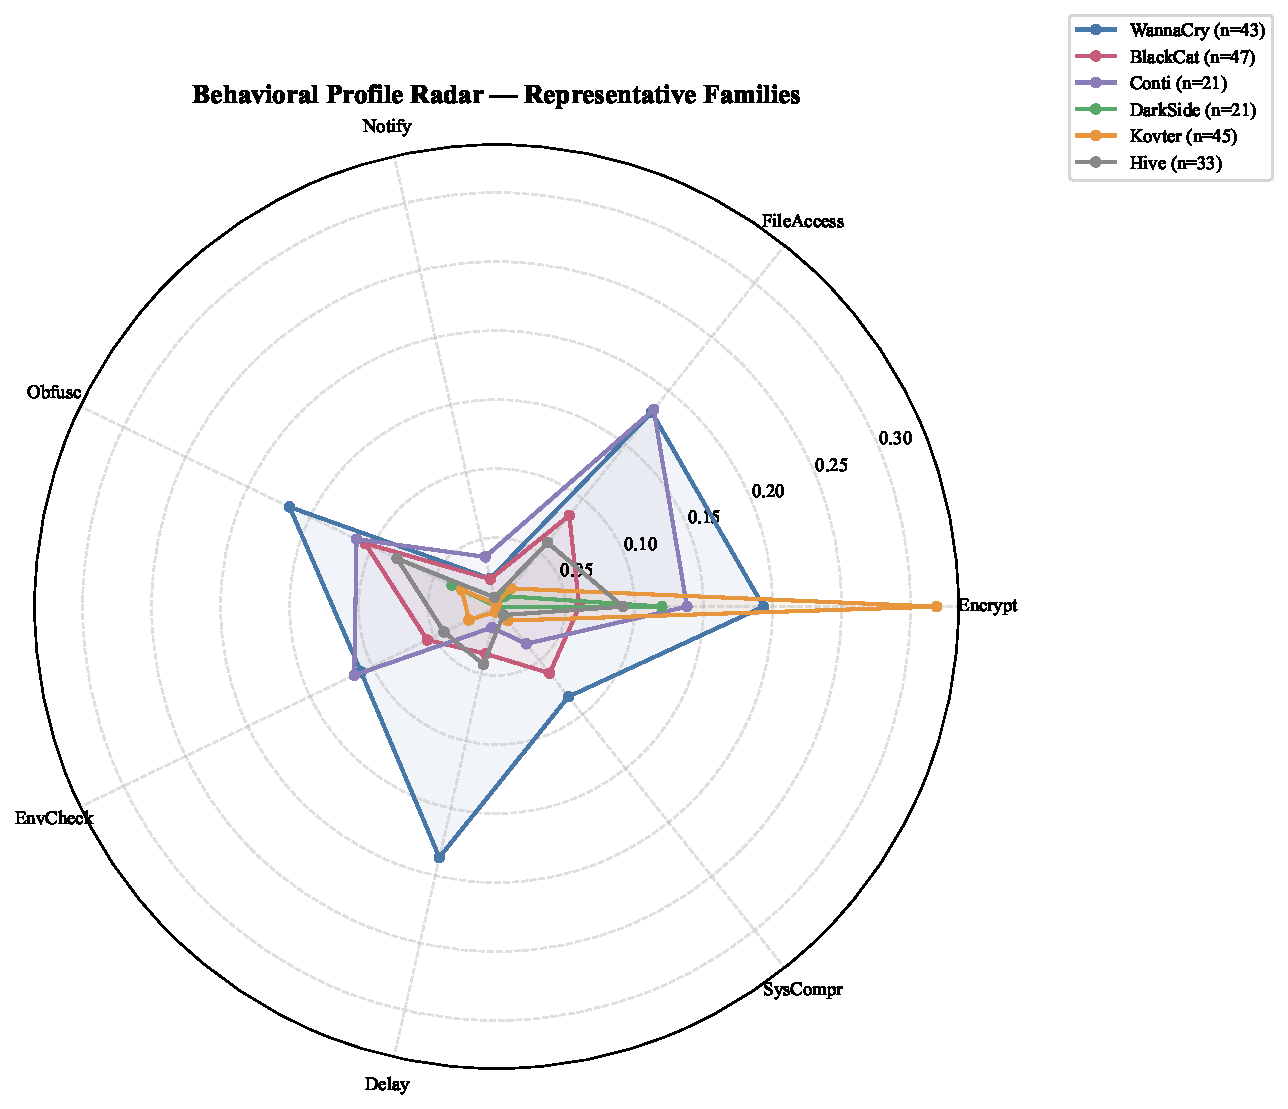
\includegraphics[width=0.95\linewidth]{figures/fig_04_rq1_radar.pdf}
\caption{代表性家族行为画像雷达图}
\label{fig:family-radar}
\end{figure}

图~\ref{fig:family-radar} 从另一个视角验证了上述判断。雷达图并未呈现“所有家族只是整体强弱不同”的同心缩放关系，而是呈现明显的方向性差异。例如，Sodinokibi 在攻击性加密与勒索展示方向上形成突出尖峰，WannaCry 在攻击性文件访问和防御性延迟执行方向同时拉伸，BlackCat 的多边形轮廓更趋于均衡而非尖锐，说明其行为更多分散到多个中等强度维度之中。正是这种“方向不同而不仅仅是幅度不同”的现象，使得行为画像能够在低维空间内保持家族判别力。

\begin{figure}[htbp]
\centering
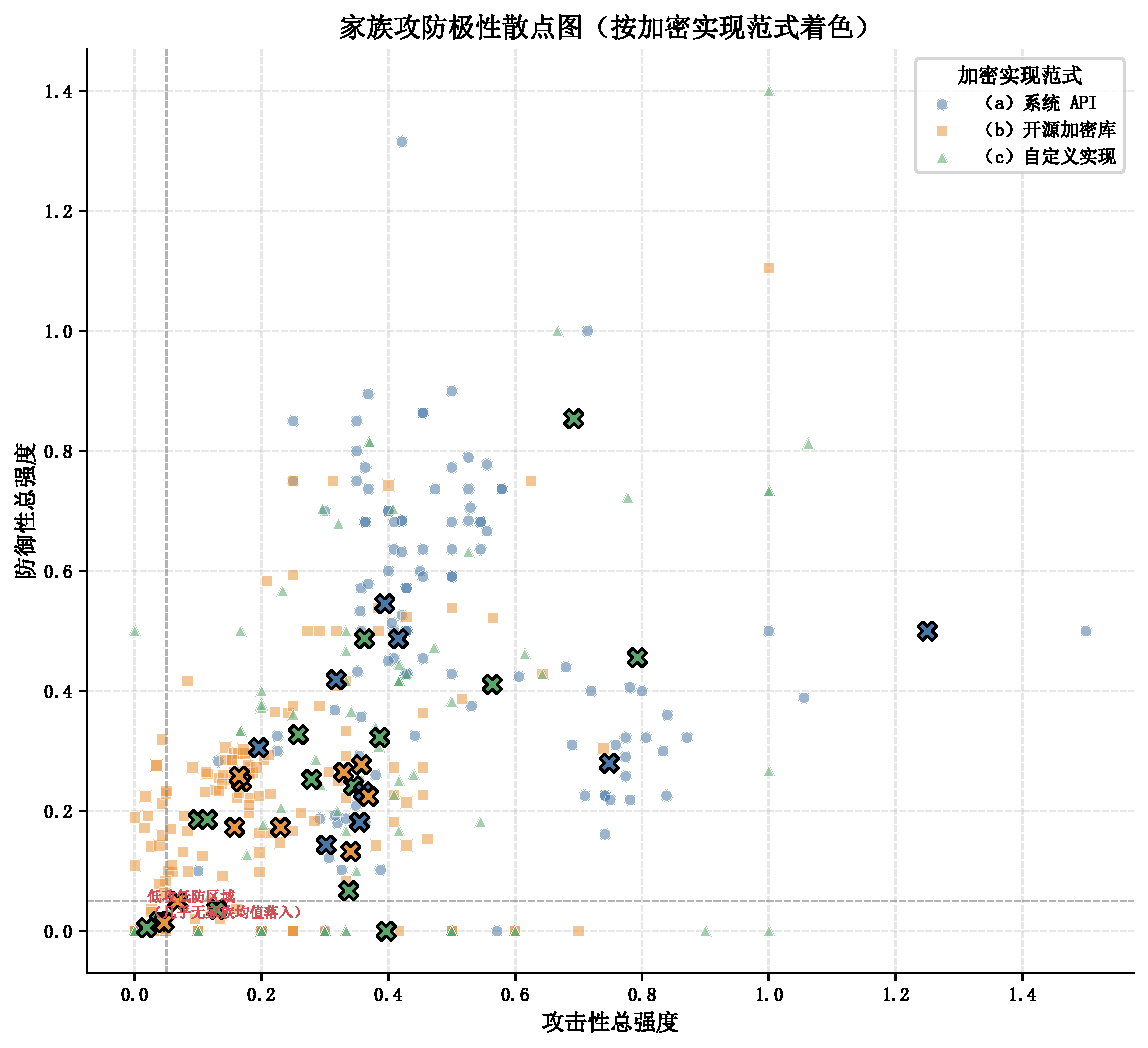
\includegraphics[width=0.95\linewidth]{figures/fig_04_rq1_polar_scatter.pdf}
\caption{家族攻防极性散点图}
\label{fig:family-polar-scatter}
\end{figure}

\subsubsection{发现 2：攻防极性约束在绝大多数家族样本上成立，二者呈准正交关系}

进一步将样本映射到攻击性强度 $O(s)$ 与防御性强度 $D(s)$ 所构成的二维空间，可以更直观地观察家族的行为组合方式。如图~\ref{fig:family-polar-scatter} 所示，不同家族在极性空间中并非随机散布，而是形成若干相对稳定的区域。Sodinokibi、Xorist 等家族集中分布在高攻击性区域，表明其主要差异来自加密与文件操作载荷的展开方式；WannaCry、Dharma、BlackCat 等家族则在攻击性和防御性之间表现出更为均衡的配置；Bianlian、Mespinoza 等家族虽然整体强度较低，但依然没有完全脱离攻防双维结构。

统计结果显示，98.2\% 的样本同时呈现攻击性与防御性行为，仅有极少数样本落入低攻击性与低防御性的边缘区域。这说明“既要完成攻击，又要保障攻击得以存活”的双重约束，并不是个别家族的偶发现象，而是跨家族普遍存在的行为组织原则。与此同时，攻击性与防御性之间的 Pearson 相关系数仅为 $r=0.48$，表明二者并非高度冗余的同一变量，而是保留了相当程度的独立变化空间。

图~\ref{fig:family-polar-scatter} 进一步说明，极性空间中的分布不是围绕一条简单主轴展开，而是表现为多个家族占据不同区域。Sodinokibi 位于高攻击性、中等防御性的右上区域，适合被解释为“载荷驱动型”家族；WannaCry 和 TeslaCrypt 虽然攻击性并不低，但在防御性方向同样向上扩展，表现出更强的执行保障需求；BlackCat 和 Hive 则落在中低攻击性、中等防御性的区域，更接近配置化、模块化的现代家族形态；Bianlian、Mespinoza 等家族靠近原点，但并未完全重合，说明即便整体行为密度较低，其攻防组合仍保留可区分差异。

这一结果具有两方面意义。其一，它解释了为何部分现代家族虽然攻击性平均值不高，却仍能通过强化环境检测、延迟执行和系统控制维持整体威胁能力。其二，它说明将全部行为压缩为单一恶意分数会不可避免地损失结构信息。对于后续识别模型而言，分别建模攻击性与防御性，不是为了增加结构复杂度，而是为了保留家族差异中的关键自由度。

\subsection{调用图关键路径的家族行为模式分析}

仅有行为占比还不足以解释家族差异的形成机制。相同的行为标签可以在完全不同的程序结构中被组织起来，因此本节进一步考察函数调用图及攻击性、 防御性子图的拓扑模式。本文分别统计全图规模、连通性、度分布和子图组织特征，并以家族分组比较其稳定性和可区分性。

\begin{figure}[htbp]
\centering
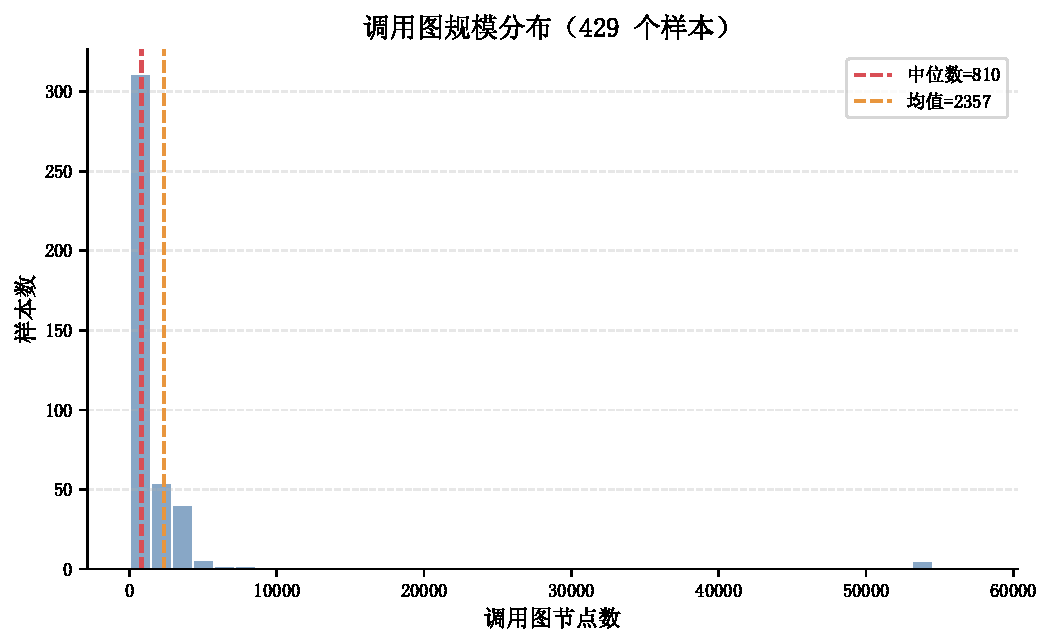
\includegraphics[width=0.95\linewidth]{figures/fig_04_rq2_graph_scale.pdf}
\caption{图规模分布直方图}
\label{fig:graph-scale}
\end{figure}

如图~\ref{fig:graph-scale} 所示，样本调用图规模呈现明显的长尾分布。大量样本聚集在相对较小的图规模区间，但仍存在一批节点数和边数极高的家族，将整体分布拉向右侧长尾。这种异质性意味着，若后续模型依赖固定大小输入或假设图规模近似稳定，则很容易在大图与小图之间产生系统性偏差。因此，在家族分析阶段先刻画图规模差异，是论证结构建模必要性的前提。

\begin{figure}[htbp]
\centering
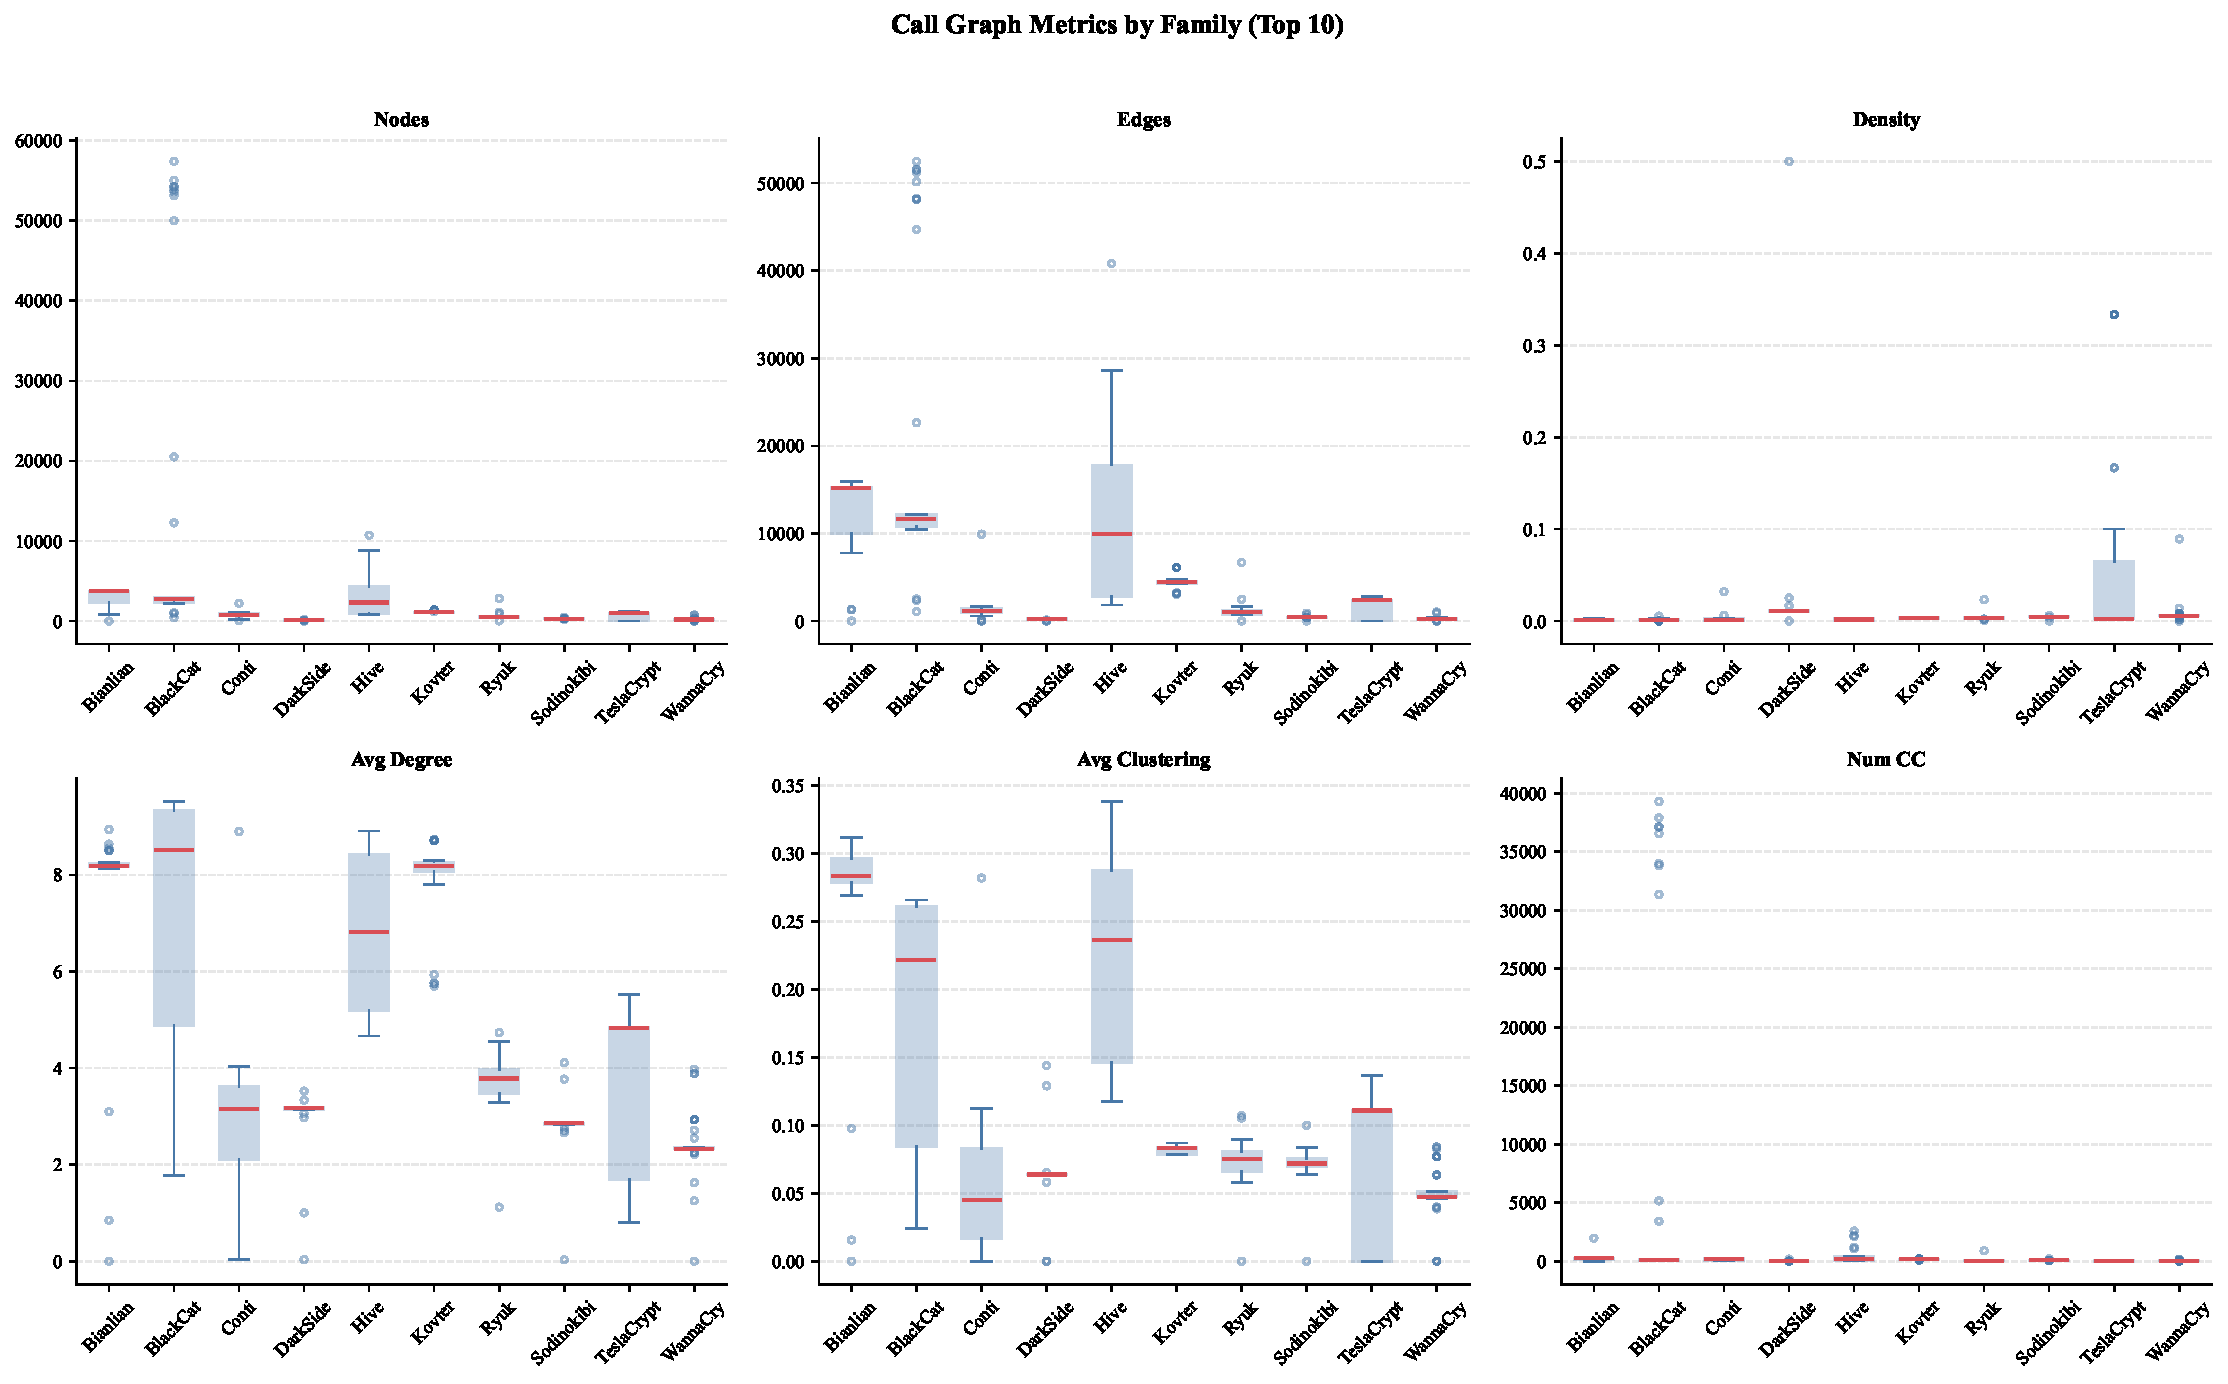
\includegraphics[width=0.95\linewidth]{figures/fig_04_rq2_callgraph_boxplots.pdf}
\caption{函数调用图拓扑指标箱线图}
\label{fig:family-callgraph-boxplot}
\end{figure}

\begin{figure}[htbp]
\centering
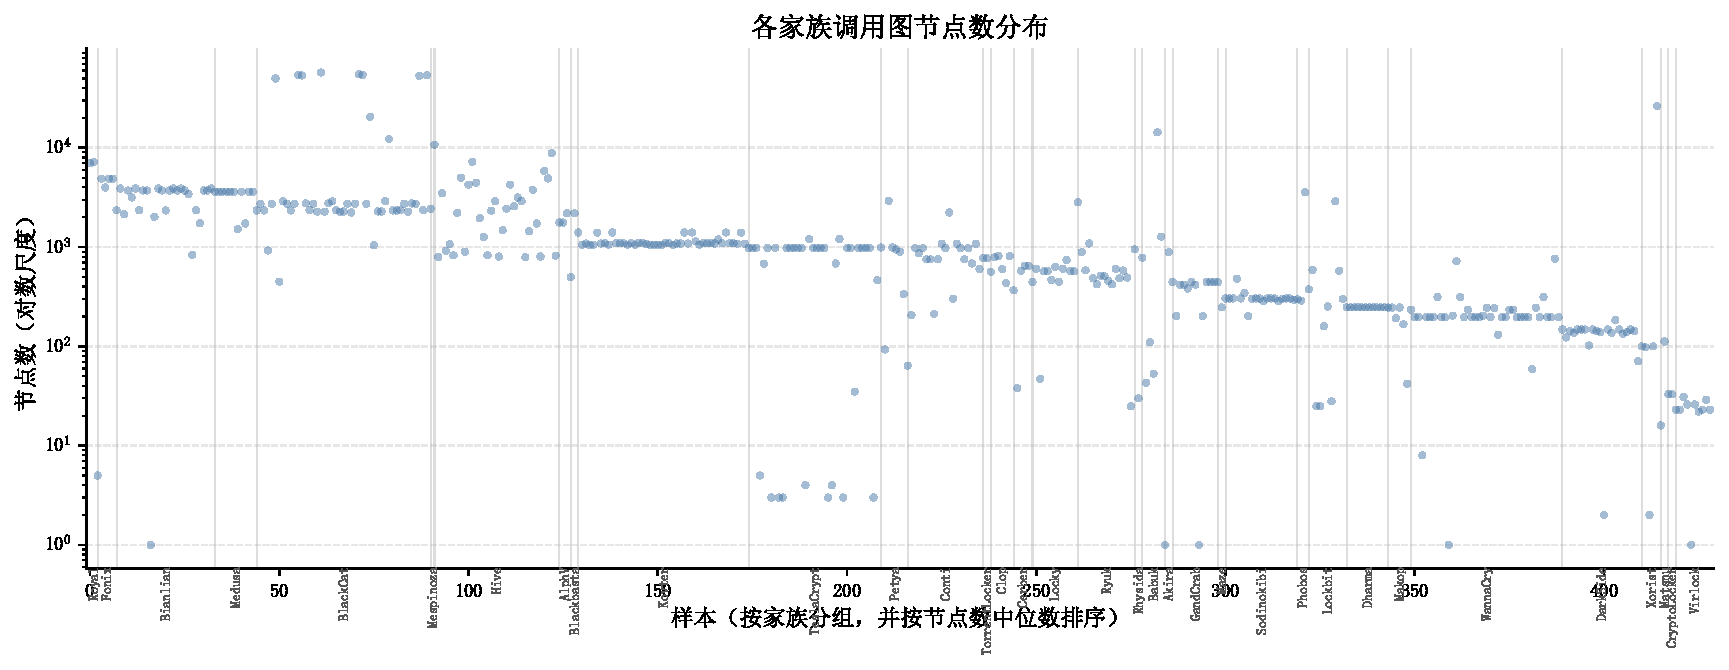
\includegraphics[width=0.95\linewidth]{figures/fig_04_rq2_nodes_by_family.pdf}
\caption{各家族节点数量分布（对数尺度）}
\label{fig:nodes-by-family}
\end{figure}

\subsubsection{发现 3：同一家族在全图拓扑上表现出更强的一致性}

对 11 项调用图拓扑指标的检验结果表明，所有指标在家族间均达到统计显著，效应量介于 0.3791 和 0.7231 之间。其中，边数和节点数的区分能力最强，$\eta^2$ 分别达到 0.7231 和 0.7035；度分布熵、平均度和密度的效应量也分别达到 0.6515、0.6107 和 0.5868。这一结果说明，不同家族在程序结构上的差异不是局部偶然现象，而是覆盖图规模、连接程度与组织复杂度的系统性差异。

进一步比较家族内与家族间的变异系数可以发现，节点数、边数、密度、平均度和度分布熵等全图指标都表现出更小的家族内波动。例如，节点数的平均家族内变异系数为 0.701，显著低于家族间变异系数 1.4413；边数对应数值为 0.7542 和 1.4111；密度对应数值为 0.7996 和 1.4650。换言之，即便家族内部存在不同编译版本和实现细节，同一家族仍会保持某种相对稳定的结构轮廓，而不同家族之间则在图规模和组织方式上拉开明显差距。

图~\ref{fig:nodes-by-family} 以对数尺度更清楚地展示了这种差距。Virlock 和 CryptoLocker 的平均节点数分别仅为 22.7 和 33.0，对应极小图家族；Dharma 和 DarkSide 的平均节点数为 247.0 和 132.4，处于中等规模但结构差异明显的区间；Sodinokibi 与 Clop 的平均节点数分别为 307.3 和 668.7，体现出较为稳定的模块化组织；BlackCat 的平均节点数高达 11961.6，Royal 为 7093.5，Bianlian、Hive 与 Medusa 也都超过 2900。可见，家族之间的程序组织复杂度已经跨越两个以上数量级，这不是单一统计阈值能够吸收的差异。

这种差异还体现在家族的结构原型上。Dharma 更接近链式结构，DarkSide、TeslaCrypt 和 Rhysida 更接近扇形或分支扩散结构，而 BlackCat、Bianlian、Hive、Medusa 等家族则更接近模块化组织方式。Virlock 与 CryptoLocker 的调用图规模明显更小，表现出简化或极小图特征。上述现象说明，家族差异并不仅仅体现为“某个函数是否出现”，而是体现为“行为被放置在怎样的程序拓扑里”。

\begin{table}[htbp]
\centering
\footnotesize
\setlength{\tabcolsep}{3.5pt}
\caption{代表性家族的调用图原型对比}
\label{tab:representative-graph-archetypes}
\begin{tabular}{lccccl}
\toprule
家族 & 平均节点数 & 平均边数 & 平均密度 & 原型 & 解释 \\
\midrule
Virlock & 22.7 & 8.0 & 0.0132 & minimal & 极小图，结构压缩明显 \\
Dharma & 247.0 & 626.0 & 0.0103 & chain-like & 链式推进，路径连续 \\
DarkSide & 132.4 & 196.2 & 0.0348 & fan-shaped & 分支扩散，局部扇出显著 \\
BlackCat & 11961.6 & 18401.8 & 0.0015 & modular & 大规模模块化组织 \\
Royal & 7093.5 & 27027.5 & 0.0005 & modular & 大图且连接稀疏 \\
\bottomrule
\end{tabular}
\end{table}

\begin{figure}[htbp]
\centering
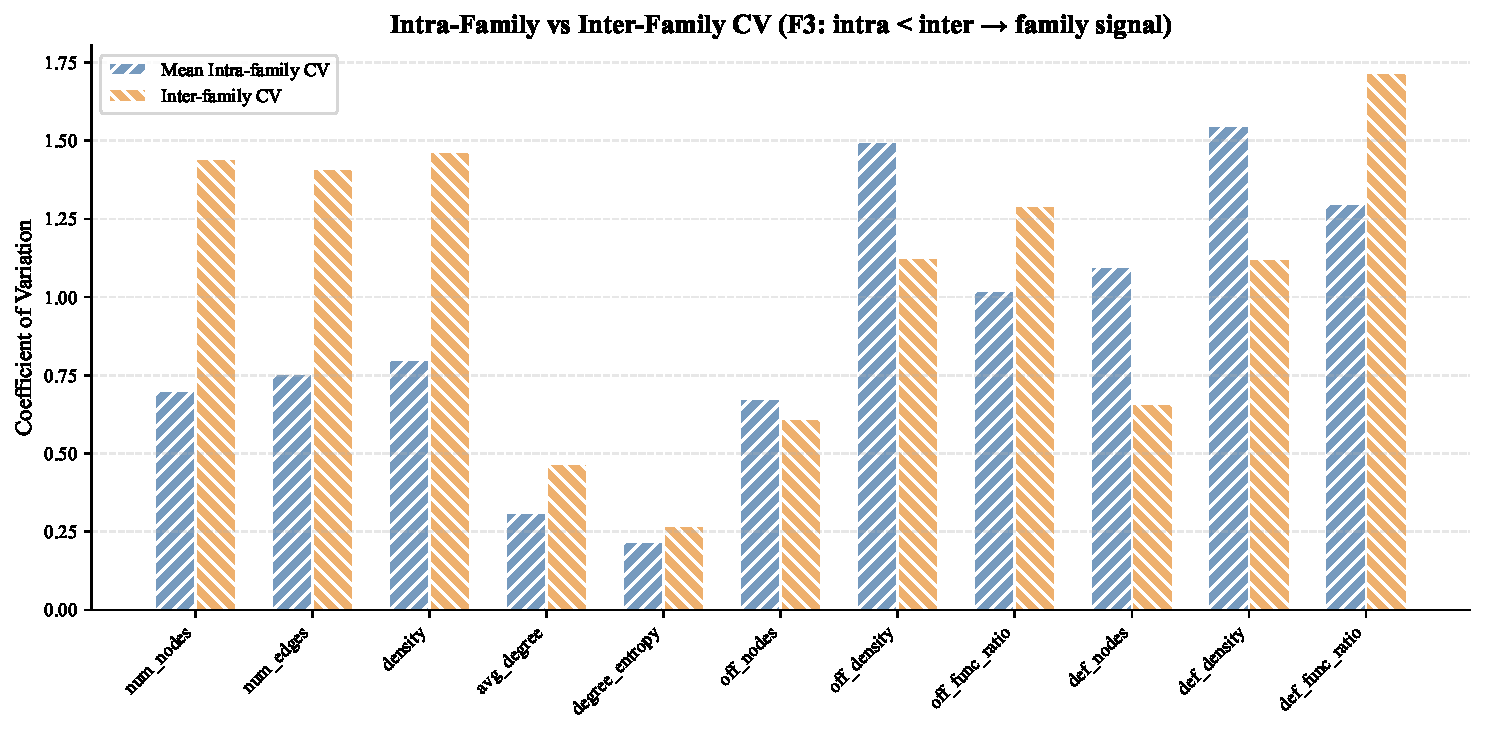
\includegraphics[width=0.95\linewidth]{figures/fig_04_rq2_cv_comparison.pdf}
\caption{五折交叉验证稳定性对比}
\label{fig:cv-comparison}
\end{figure}

图~\ref{fig:cv-comparison} 给出了家族内和家族间变异系数的直接对照。从统计结果看，11 个指标中有 7 个满足“家族内变异小于家族间变异”，其中节点数、边数、密度、平均度和度分布熵这五个全图指标最为稳定；与之相比，\textit{off\_nodes}、\textit{off\_density}、\textit{def\_nodes} 和 \textit{def\_density} 四个指标表现出更高的家族内波动，说明攻击性、 防御性子图的局部规模更容易受到版本差异和功能裁剪影响。这一现象并未削弱家族可区分性，反而提示：全图拓扑更适合作为家族稳定背景，而 O/D 子图拓扑更适合作为刻画家族内部执行策略变化的补充视角。

\begin{table}[htbp]
\centering
\footnotesize
\setlength{\tabcolsep}{4pt}
\caption{攻击性与防御性子图的关键拓扑差异}
\label{tab:od-topology-diff}
\begin{tabular}{lcccc}
\toprule
指标 & 攻击性均值 & 防御性均值 & $p$ 值 & 差异方向 \\
\midrule
节点数 & 8.2652 & 6.3068 & $4.56\times10^{-8}$ & 攻击性更大 \\
连通分量数 & 6.5720 & 4.9545 & $9.22\times10^{-8}$ & 攻击性更分散 \\
密度 & 0.0260 & 0.0436 & $2.64\times10^{-3}$ & 防御性更紧致 \\
最大连通分量比例 & 0.3287 & 0.4162 & $4.64\times10^{-7}$ & 防御性更集中 \\
最大介数中心性 & 0.0039 & 0.0091 & $9.67\times10^{-4}$ & 防御性瓶颈更明显 \\
\bottomrule
\end{tabular}
\end{table}

\begin{figure}[htbp]
\centering
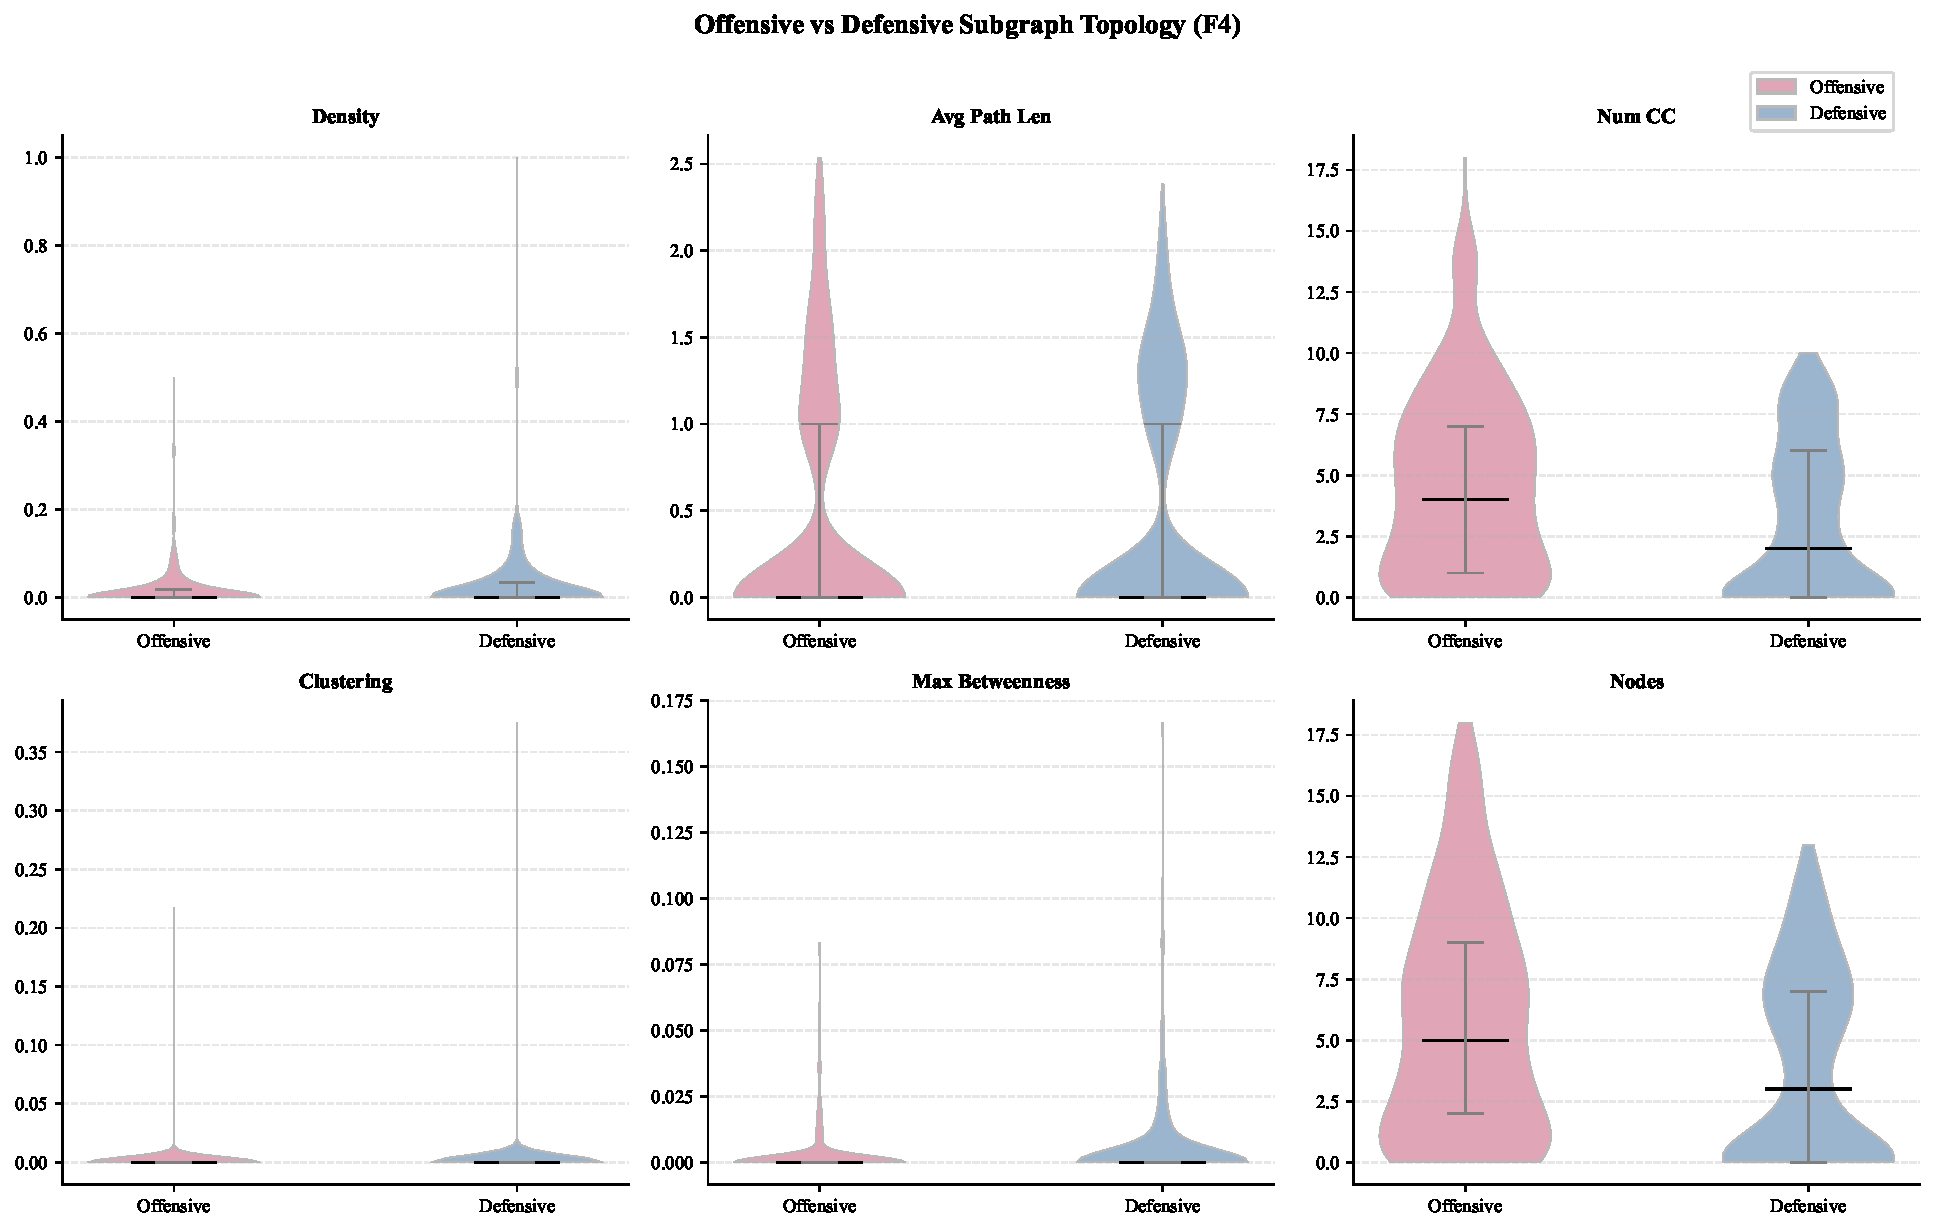
\includegraphics[width=0.95\linewidth]{figures/fig_04_rq2_od_violin.pdf}
\caption{攻击性/防御性子图拓扑小提琴图}
\label{fig:od-violin}
\end{figure}

\subsubsection{发现 4：攻击性子图更分散，防御性子图更紧致}

表~\ref{tab:od-topology-diff} 和图~\ref{fig:od-violin} 共同揭示了攻击性与防御性子图在组织方式上的稳定差异。攻击性子图的平均节点数为 8.2652，高于防御性子图的 6.3068；平均连通分量数为 6.5720，也高于防御性子图的 4.9545。这表明攻击性逻辑更常分散在多条执行路径之中，例如加密、文件遍历和勒索展示可能分别由不同的函数簇触发，其间联系较弱，更多体现为并列展开的多路径结构。

与之相对，防御性子图虽然规模较小，但在密度、最大连通分量比例和最大介数中心性上均显著高于攻击性子图。防御性子图的平均密度达到 0.0436，高于攻击性子图的 0.0260；最大连通分量比例为 0.4162，也明显高于攻击性子图的 0.3287；最大介数中心性为 0.0091，高于攻击性子图的 0.0039。这说明防御性逻辑更倾向于围绕少量关键节点形成集中式组织，例如环境检查、反调试和触发条件控制往往需要在执行早期共同决定是否继续展开攻击载荷，因此其结构更像一个小而紧密的“规避核心”。

值得注意的是，并非所有拓扑指标都表现出同等显著性。平均路径长度和聚类系数在攻击性与防御性子图之间差异不显著，说明二者的区别并不是简单地体现在每一个图指标上，而是主要体现在规模、连通性和关键节点组织方式上。换言之，家族差异并不来自“攻击性图一定更长”或“防御性图一定更聚类”这类单一规律，而来自多个局部统计同时偏移所形成的综合结构模式。这种差异模式为第五章的双图建模提供了直接启发：如果攻击性子图承担的是多路径展开模式，而防御性子图承担的是关键节点控制模式，那么将二者分离编码比在单图中混合学习更有可能保留结构差异。与此同时，样本调用图规模从几十个节点到上万个节点不等，这也解释了为何后续更适合采用具备归纳式邻居采样能力的 GraphSAGE 结构 \cite{hamilton2017inductive}。

\subsection{知识库三层特征的家族覆盖与判别力}

在行为画像和拓扑结构之外，本章还需要回答一个更基础的问题：第三章提出的三层知识体系究竟在多大程度上覆盖了不同家族的真实行为差异。为此，本节同时从“是否命中”与“命中强度”两个层面审计词法层、语义层和统计层，并进一步比较 54 个可比统计特征及其特征组的家族判别能力。

\begin{figure}[htbp]
\centering
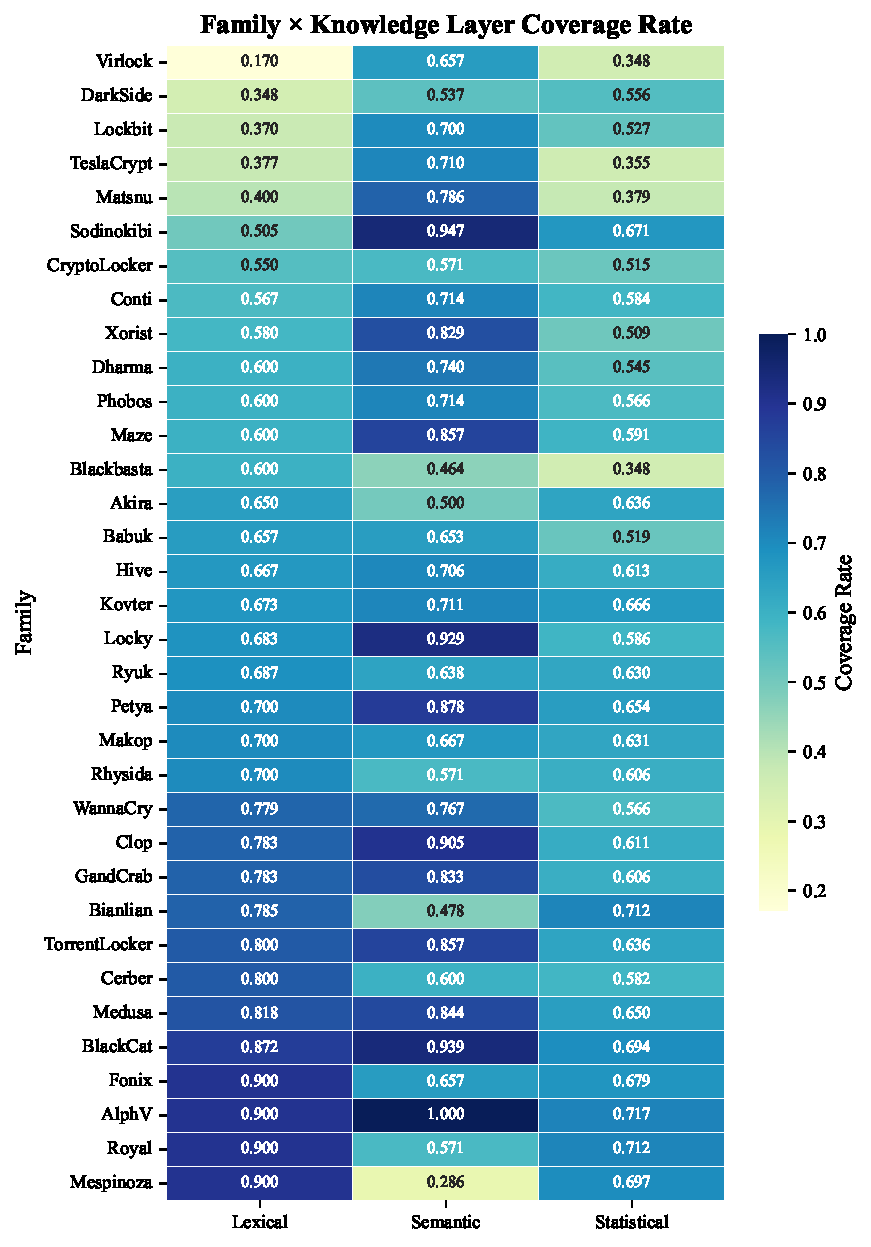
\includegraphics[width=0.95\linewidth]{figures/fig_04_rq3_coverage_heatmap.pdf}
\caption{三层知识在不同家族上的覆盖热力图}
\label{fig:kb-coverage-heatmap}
\end{figure}

\subsubsection{发现 5：三层知识在粗粒度覆盖上接近完备，在命中强度上体现明显互补}

从样本是否被某层知识捕获这一粗粒度标准看，词法层和统计层对 34 个家族均达到 100\% 的样本级覆盖，语义层也对绝大多数家族保持较高覆盖率，仅在 Akira、Blackbasta 和 TeslaCrypt 等少数家族上有所下降，其中 Akira 和 Blackbasta 的语义层覆盖率为 50.0\%，TeslaCrypt 为 74.29\%，WannaCry 为 86.05\%。这意味着，第三章构建的三层知识体系在“是否能够触达家族行为”这一层面已经具备较强普适性，并不存在大面积完全失效的家族盲区。

然而，真正体现层间差异的并不是“是否命中”，而是“命中强度”。以各家族的平均命中比例为例，Virlock 的词法层命中强度仅为 0.17，而语义层达到 0.6571，说明其多态与轻量化实现方式削弱了字面证据，却保留了可以被语义规则识别的行为模式；Sodinokibi 的词法层和语义层命中强度分别为 0.5053 和 0.9474，Lockbit 分别为 0.37 和 0.70，TeslaCrypt 分别为 0.3771 和 0.7102，均表现出语义层对复杂家族的明显补偿作用。与之相反，Mespinoza 的语义层命中强度仅为 0.2857，而词法层和统计层分别达到 0.90 和 0.697，说明极小样本与简化实现可能更依赖字面证据和数值指纹。

结合相关性分析可知，词法层与语义层的覆盖强度相关系数仅为 $r=0.06$，说明二者并非简单重复，而是在不同家族上承担不同识别任务。换言之，三层知识体系并不是把同一证据重复编码三次，而是通过差异化描述机制分别触达不同家族的行为侧面。这一结论为第三章知识库的分层设计提供了直接支撑，也说明后续识别模型有必要同时保留字面、语义和统计三类输入，而不是过早合并为单一特征空间。

图~\ref{fig:kb-coverage-heatmap} 所呈现的并不是“哪一层完全覆盖、哪一层完全缺失”的二元格局，而是不同家族在三层命中强度上的梯度变化。以 Virlock 为例，其词法层命中强度仅为 0.17，但语义层达到 0.6571，说明该家族在字面层面高度稀疏，却保留了可被语义规则恢复的行为模式；Sodinokibi 的语义层命中强度达到 0.9474，显著高于词法层的 0.5053；TeslaCrypt 的语义层命中强度为 0.7102，也明显高于词法层的 0.3771。相反，Mespinoza 的语义层命中强度仅为 0.2857，而词法层和统计层分别达到 0.90 和 0.697，说明极小样本与简化实现并不一定受益于更复杂的语义规则。这些具体例子表明，三层知识的互补关系必须通过家族差异来理解，而不能仅凭整体平均值判断。

\begin{figure}[htbp]
\centering
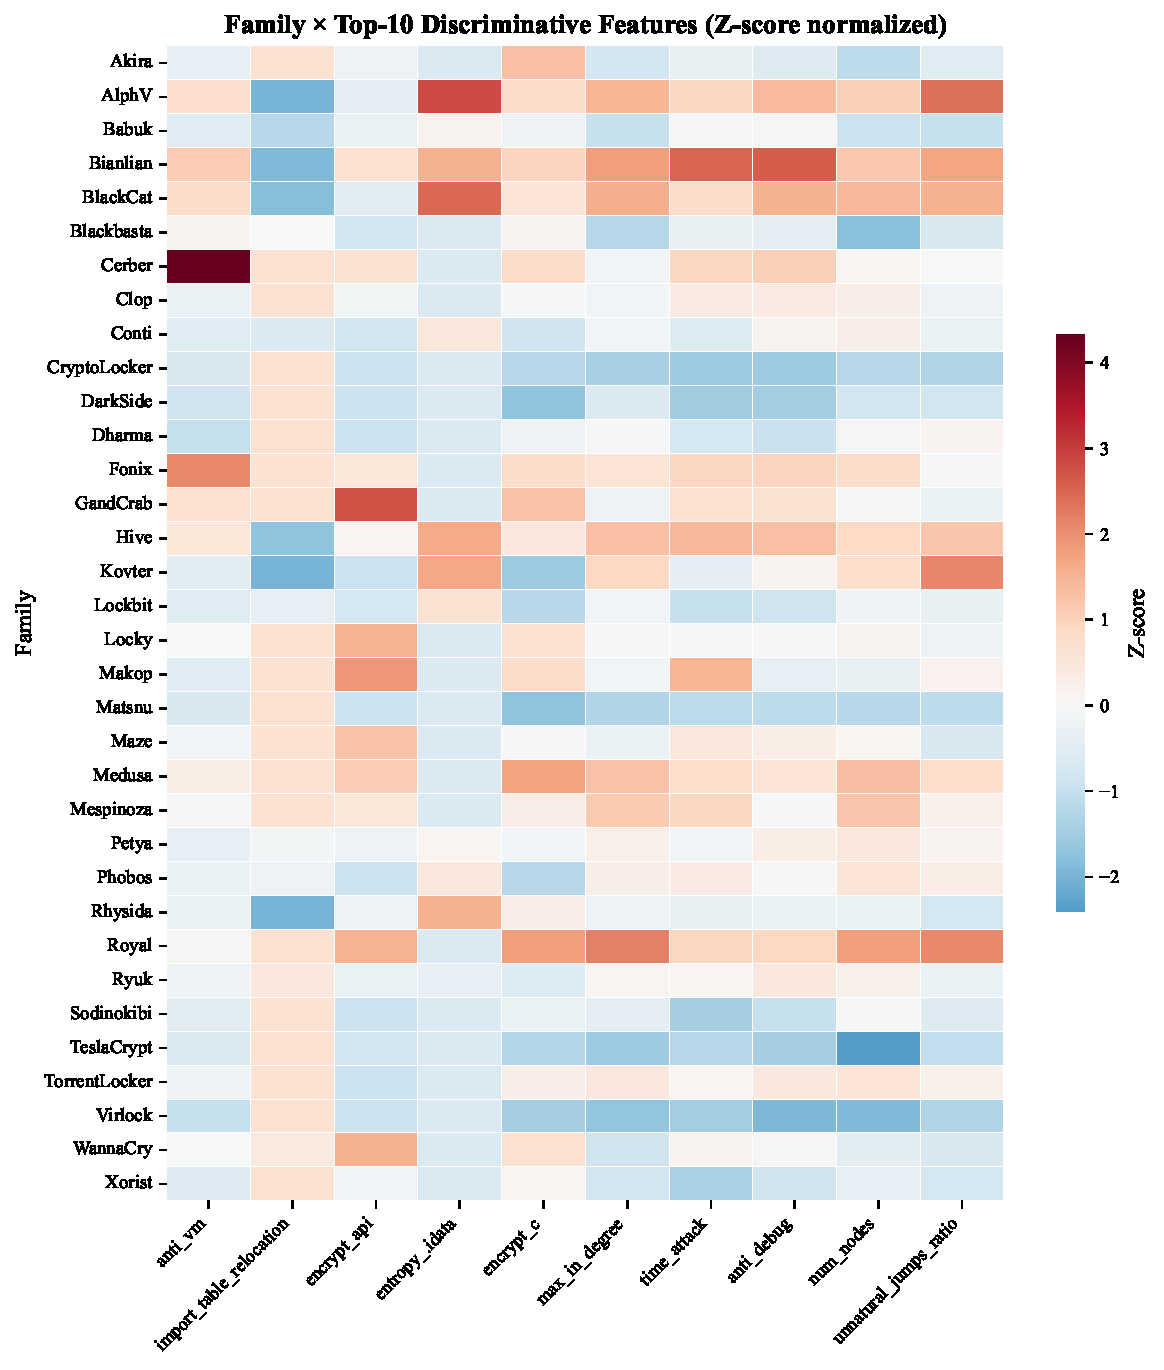
\includegraphics[width=0.95\linewidth]{figures/fig_04_rq3_feature_heatmap.pdf}
\caption{特征值分布热力图}
\label{fig:feature-heatmap}
\end{figure}

图~\ref{fig:feature-heatmap} 进一步说明，真正驱动家族分离的不只是“某层命中了多少次”，还包括不同高判别力特征在家族之间形成的稳定高低带。例如，反分析类特征、加密 API 类特征与部分 PE 结构特征并未在所有家族上均匀激活，而是在若干家族上形成明显高值条带。热力图中的这种条带结构意味着，家族可区分性不是来自某个单一阈值，而是来自多个特征在不同家族上的协同组合。

\begin{figure}[htbp]
\centering
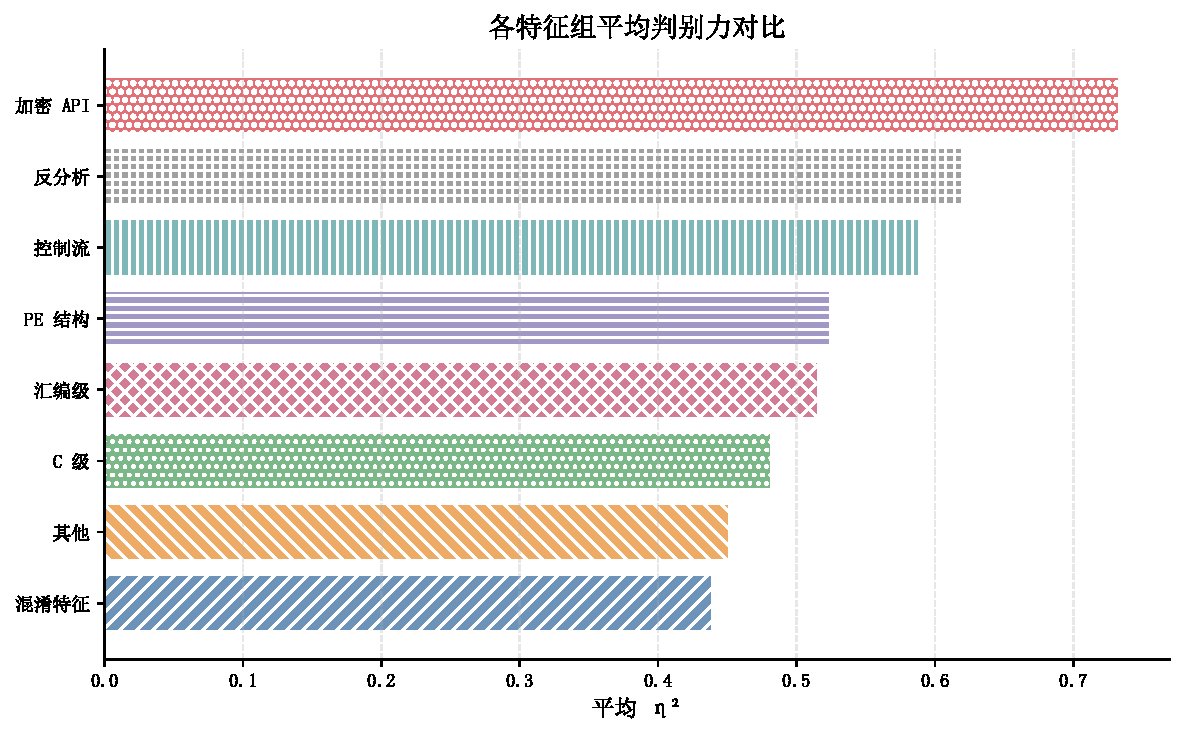
\includegraphics[width=0.95\linewidth]{figures/fig_04_rq3_group_discriminability.pdf}
\caption{特征组判别力对比}
\label{fig:group-discriminability}
\end{figure}

\begin{table}[htbp]
\centering
\footnotesize
\setlength{\tabcolsep}{4pt}
\caption{主要特征组的平均家族判别力}
\label{tab:feature-group-discriminability}
\begin{tabular}{lcc}
\toprule
特征组 & 特征数 & 平均 $\eta^2$ \\
\midrule
加密 API 特征 & 2 & 0.7332 \\
反分析特征 & 6 & 0.6200 \\
控制流特征 & 8 & 0.5885 \\
PE 结构特征 & 17 & 0.5242 \\
汇编级特征 & 9 & 0.5158 \\
C 级特征 & 4 & 0.4815 \\
\bottomrule
\end{tabular}
\end{table}

\subsubsection{发现 6：统计特征为家族比较提供最强的细粒度判别信号}

在 54 个可比较统计特征中，除 \texttt{entropy\_.edata} 之外，其余 53 个特征均达到显著的大效应水平，说明统计层并非对行为画像的简单补充，而是能够在更细粒度上形成家族“数值指纹”。从单个特征看，判别力最强的五个指标分别为 \texttt{anti\_vm}（$\eta^2=0.7685$）、\texttt{import\_table\_relocation}（$\eta^2=0.7640$）、\texttt{encrypt\_api}（$\eta^2=0.7495$）、\texttt{entropy\_.idata}（$\eta^2=0.7448$）和 \texttt{encrypt\_c}（$\eta^2=0.7168$）。这些指标分别对应反分析能力、导入表组织方式、加密接口调用以及节区结构异常，表明家族差异已经深刻嵌入到程序布局和执行准备过程之中。

\begin{figure}[htbp]
\centering
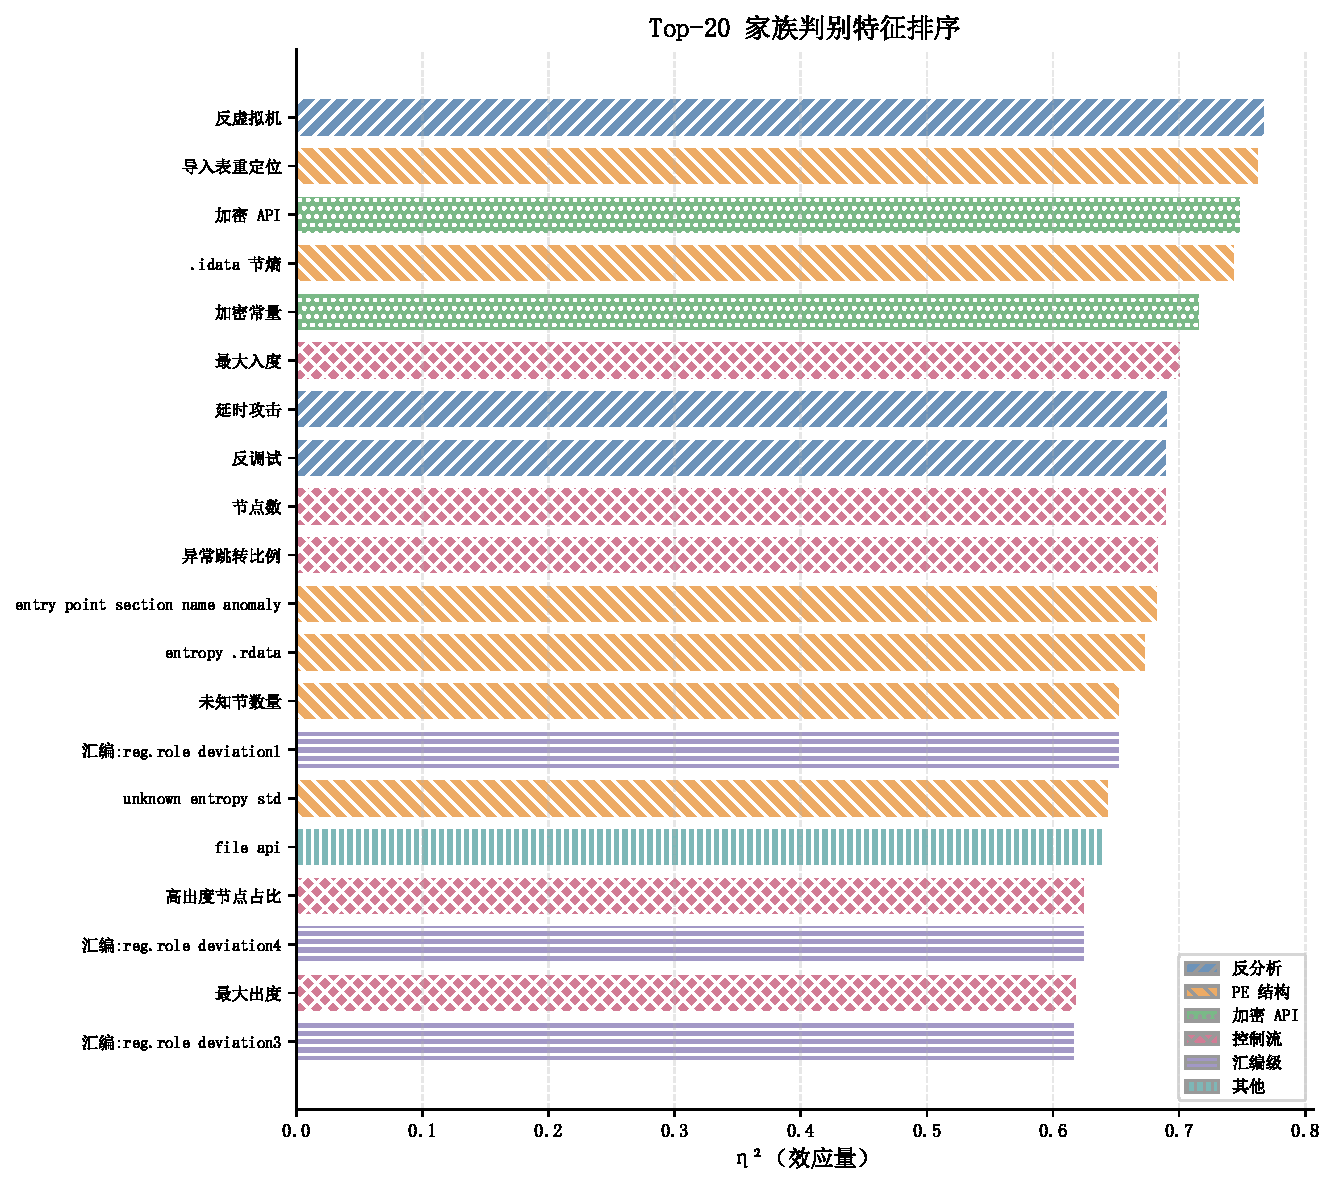
\includegraphics[width=0.95\linewidth]{figures/fig_04_rq3_importance_top20.pdf}
\caption{Top-20 特征判别力排序}
\label{fig:importance-top20}
\end{figure}

\begin{table}[htbp]
\centering
\footnotesize
\setlength{\tabcolsep}{4pt}
\caption{Top-6 家族判别力最强的统计特征}
\label{tab:top-discriminative-features}
\begin{tabular}{lccc}
\toprule
特征 & 特征组 & $\eta^2$ & Fisher score \\
\midrule
\texttt{anti\_vm} & Anti-analysis & 0.7685 & 4.0018 \\
\texttt{import\_table\_relocation} & PE-structure & 0.7640 & 3.5845 \\
\texttt{encrypt\_api} & Encryption-API & 0.7495 & 3.0481 \\
\texttt{entropy\_.idata} & PE-structure & 0.7448 & 3.0224 \\
\texttt{encrypt\_c} & Encryption-API & 0.7168 & 2.9724 \\
\texttt{max\_in\_degree} & Control-flow & 0.7018 & 2.3566 \\
\bottomrule
\end{tabular}
\end{table}

从特征组层面看，表~\ref{tab:feature-group-discriminability} 表明加密 API 特征的平均判别力最高，达到 0.7332；反分析特征和控制流特征紧随其后，分别为 0.6200 和 0.5885；PE 结构、汇编级和 C 级特征也都维持在 0.48 以上的大效应水平。这说明，统计层之所以能够成为家族比较中最强的细粒度信号，并不只因为某一个“强特征”异常突出，而是因为多个特征组都在不同角度刻画了家族的实现风格。

图~\ref{fig:importance-top20} 与表~\ref{tab:top-discriminative-features} 对这一点给出了更细的证据。Top-20 特征并未集中在单一组别，而是横跨反分析、PE 结构、加密 API、控制流和汇编级多个维度。尤其是 \texttt{anti\_vm}、\texttt{encrypt\_api} 与 \texttt{import\_table\_relocation} 这三类特征分别对应环境规避、加密执行入口和导入表布局异常，说明家族差异同时体现在运行前规避、运行中载荷调用和静态布局痕迹三个层级上。换言之，统计层之所以判别力强，并不是因为它“更高维”，而是因为它把多个层面的实现偏好叠加到了同一数值空间中。

这一发现与前两节结论形成互补关系：如果说七维行为画像回答了“家族做什么”，调用图拓扑回答了“家族如何组织这些行为”，那么统计特征进一步回答了“这些行为通过怎样的底层实现痕迹表现出来”。因此，统计层在后续识别模型中不应被视为附属通道，而应作为与图结构表征并行的重要信息源。

\subsection{本章小结}

本章围绕勒索软件家族在行为语义、调用图结构和知识证据覆盖上的差异展开系统分析，形成了六项彼此衔接的发现。发现 1 表明，七维攻防行为画像已经足以稳定区分 34 个家族；发现 2 说明，攻击性与防御性共同构成跨家族普遍成立的双维约束，且二者保留准正交关系；发现 3 与发现 4 进一步揭示，家族差异不仅存在于行为内容，也存在于调用图的组织方式之中，其中攻击性子图更分散、防御性子图更紧致；发现 5 与发现 6 则说明，三层知识体系在粗粒度覆盖上接近完备，在命中强度和细粒度统计判别力上体现出明确互补。

这些结果共同说明，家族可区分性并非由单一证据源驱动，而是由行为组合、图结构和数值实现痕迹共同构成的复合现象。对第五章而言，本章最直接的启示有两点：其一，攻击性与防御性信息应保留分离建模；其二，图结构表征与统计特征表征应联合输入，而不是以其中任一方替代另一方。由此，第四章完成了从行为语义到结构建模之间的桥接，为后续双图语义神经网络的设计提供了经验依据。